\section{数据重发}
\subsection{简述数据重发}
TCP使用定时器函数tcp\_retransmit\_timer进行数据重发,MPTCP需要重发数据的时候,不仅仅在原路径发送数据,而且会在另外一条子路径进行重发。这样考虑的原因是:考虑网络中间件设备的影响, 保证子路径上数据序列号的完整性。目前的版本0.89依然如此实现,以后应该会优化。
\subsection{内核实现}
MPTCP的结构如下图所示:
\begin{figure}[H]
  \centering
  % Requires \usepackage{graphicx}
  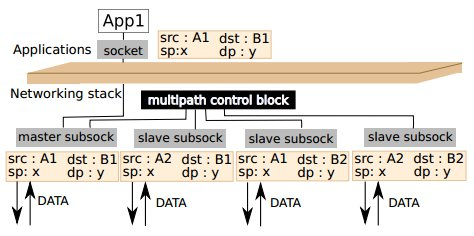
\includegraphics[width=10cm]{dias/Kernal.jpg}\\
  \caption{MPTCP的结构图}
\end{figure}
如上图所示:每一个slave subsock 和 master subsock实际上维持着一个正常的TCP链路,因此,他们都具有重发定时器tcp\_write\_timer。MPTCP实现的思路就是:每个子链路发送失败的时候,将发送失败的SKB拷贝一份到meta sock。然后让meta sock 再次选择另外一条子路径发送。

如下是对tcp\_retransmit\_timer的修改:
\small\begin{verbatim}
"net/ipv4/tcp_timer.c"  line 488 of 691
487
488 out:;
489     if (mptcp(tp)) {
490         mptcp_reinject_data(sk, 1);
491         mptcp_set_rto(sk);
492     }
493 }
\end{verbatim}\normalsize
函数mptcp\_reinject\_data的实现如下:
\small\begin{verbatim}
"net/mptcp/mptcp_output.c" line 237 of 1667
236 /* Inserts data into the reinject queue */
237 void mptcp_reinject_data(struct sock *sk, int clone_it)
238 {
239     struct sk_buff *skb_it, *tmp;
240     struct tcp_sock *tp = tcp_sk(sk);
241     struct sock *meta_sk = tp->meta_sk;
242
243     /* It has already been closed - there is really no point in reinjecting */
244     if (meta_sk->sk_state == TCP_CLOSE)
245         return;
246
247     skb_queue_walk_safe(&sk->sk_write_queue, skb_it, tmp) {
248         struct tcp_skb_cb *tcb = TCP_SKB_CB(skb_it);
249         /* Subflow syn's and fin's are not reinjected.
250          *
251          * As well as empty subflow-fins with a data-fin.
252          * They are reinjected below (without the subflow-fin-flag)
253          */
254         if (tcb->tcp_flags & TCPHDR_SYN ||
255             (tcb->tcp_flags & TCPHDR_FIN && !mptcp_is_data_fin(skb_it)) ||
256             (tcb->tcp_flags & TCPHDR_FIN && mptcp_is_data_fin(skb_it) && !skb_it->len))
257             continue;
258
259         __mptcp_reinject_data(skb_it, meta_sk, sk, clone_it);
260     }
261
262     skb_it = tcp_write_queue_tail(meta_sk);
263     /* If sk has sent the empty data-fin, we have to reinject it too. */
264     if (skb_it && mptcp_is_data_fin(skb_it) && skb_it->len == 0 &&
265         TCP_SKB_CB(skb_it)->path_mask & mptcp_pi_to_flag(tp->mptcp->path_index)) {
266         __mptcp_reinject_data(skb_it, meta_sk, NULL, 1);
267     }
268
269     mptcp_push_pending_frames(meta_sk);
270
271     tp->pf = 1;
272 }
\end{verbatim}\normalsize
第259行的\_\_mptcp\_reinject\_data函数将出现超时的sk$\rightarrow$sk\_write\_queue的数据拷贝到 meta\_sk 的reinject queue。\\
而269行的函数mptcp\_push\_pending\_frames将会对reinject queue中的数据进行发送,其调用关系如下:
\small\begin{verbatim}
    mptcp_push_pending_frames
                            =》__tcp_push_pending_frames
                                 =》tcp_sk(sk)->write_xmit
                                      =》mptcp_write_xmit
                                           =》mptcp_next_segment
                                                =》__mptcp_next_segment
                                                =》get_available_subflow
\end{verbatim}\normalsize
\subsection{结论}
\begin{itemize}
  \item 子路径出现重发数据的情况下,MPTCP会选择另外一条路径发送同样的数据。
\end{itemize}